\documentclass[a4paper, 12pt] {article}
%\usepackage[pd,col,3d,turt]{mgtex_23}
\usepackage{etex}
\usepackage[utf8]{inputenc}
\usepackage[T1]{fontenc}
\usepackage{amssymb}
\usepackage{amsthm}
\usepackage{amsmath}
\usepackage[ruled,vlined]{algorithm2e}
\usepackage{graphicx}
\usepackage{todonotes}
\usepackage{pgfplots}


\newtheoremstyle{example}
     {\topsep}%      Space above
     {\topsep}%      Space below
     {}%         Body font
     {}%         Indent amount (empty = no indent, \parindent = para indent)
     {\bfseries}% Thm head font
     {}%        Punctuation after thm head
     {}%     Space after thm head: " " = normal interword space;
           %       \newline = linebreak
     {\underline{\thmname{#1}\thmnumber{ #2}\thmnote{ (#3)}}}%         Thm head spec (can be left empty, meaning `normal')
%     \theoremstyle{example}
     \newtheorem*{example}{Example}
\newtheorem*{Note}{Note}
\begin{document}
\listoftodos
\newpage
\title{Advanced Methods in Stochastic Programming}
\author{Hans Pirnay}
\maketitle
\tableofcontents
\newpage
\section{Introduction}
\todo{write an introduction}
\section{Stochastic Programming Theory}
Consider the following real world problem:

An operator in charge of a pumped hydro plant at any given time wants to make the optimal decision wether to pump water up into hhis reservoir with electrical power purchased at current spot market prices, do nothing, or release water from the reservoir and sell it at the spot market. 

For an introduction into the general theory see \cite{Birge1997}. For a more recent overview on optimization under uncertainty, see \cite{Sahinidis2004} and the references therein.
% here, explain the following terms:
% - value of the stochastic solution
% - perfect foresight
% - here and now / wait and see
\section{Scenario tree generation}
The generation of the scenario tree is a key step in the solution of stochastic programming problems.

In this section we will present several ways to generate said scenario trees. The section is organized as follows. First, I will give an short introduction to the basic mathematical theory necessary to follow the derivations of the algorithms. Then, the state of the art in solving this problem is summarized. Finally, three new algorithms are derived. These new algorithms will differ from the ones proposed in the literature in that they attempt to actually solve the original problem to full optimality. The section will close with a discussion and comparision of the results of the presented algorithms. 
\subsection{Mathematical Foundations}
This section serves as a short introduction to the mathematical concepts used throughout this paper. The reader should be familiar with the most basic concepts of probability theory and measure theory, such as probability spaces, sigma algebras, filtration and measures.

This section is organized as follows. First, the above description of a real world problem is tranlated into the context and notation of probability theory. Then the resulting abstract mathematical description is transformed into a numerically tangible formulation.
\subsubsection{Notation}
We will only deal with stochastic processes with discrete time steps. These time steps will be indexed from 1 to a final time T. For a stochastic process $\xi$ with a continuous distribution, $\xi^t$ denotes the mapping from events to outcomes at timestep $t$. For discrete stochastic processes, index sets for the events, typically denoted by $I$ and $J$, are introduced. The outcome of event $i\in I$ of a discrete stochastic process $\xi$ at timestep $t$ is denoted by $\xi_i^t$. If the timestep is omitted, this denotes the full scenario $i$, that is the vector of the values $\xi_i^t$ sorted by their times $t$.
\subsubsection{Stochastic Programming and Scenario Trees}
Suppose a problem given in the following generic nonlinear multi-stage stochastic programming problem. 
\begin{eqnarray}
  \label{eq:genericSP}
  \min &&\mathbb{E}\left[\sum_{t=1}^Tf_t(\xi_t, x_t)\right]\\
  &\mathrm{s.t.}& h_t(\xi_t, x_t, x_{t-1}) = 0\\
  &&x_t \in X_t\\
  &&x_t \, \mathrm{is}\,\mathcal{F}_t \mathrm{-measurable} \label{eqn:measurability-constraint}
\end{eqnarray}
In this problem, the stochastic process $\xi$ can be considered as a mapping $\xi:\Omega\rightarrow \mathbb{R}^{d\times T}$, where $\Omega$ is the sample space of the underlying probability space $(\Omega, \mathcal{F}, \mathbb{P})$. The solution is a mapping $x:\Omega\rightarrow \mathbb{R}^{n\times T}$.
 
The difficulty in multi-stage stochastic programming problems arises from the measurability constraint (\ref{eqn:measurability-constraint}). This constraint is specific to multi-stage stochastic programs, since in two-stage stochastic programs, there are no future states associated with uncertain states. This additional constraint leads to a much increased computational complexity of multi-stage programs over two-stage programs \cite{Shapiro2005,Shapiro2008}. Practically, this constraint means that the condition
\begin{equation}
  \label{eq:mathematical_NAC}
  \omega_1,\omega_2\in \Omega \, : \, \xi_\tau(\omega_1) = \xi_\tau(\omega_2)\,\forall \tau\leq t\,\Rightarrow \, x_t(\omega_1) = x_t(\omega_2) 
\end{equation}
has to hold for all time steps $t$, and all pairs of events $(\omega_1,\omega_2)$. The decision variables $x_t$ must only depend on the events of the past up until the present $\xi_1$, ..., $\xi_t$, and explicitly \textbf{not} on $xi_{t+1},\, ...,\,\xi_T$. This property is often called \textit{non-anticipativity of the solution} $x$. Therefore, these equations model the uncertainty of the future.

To transform the stochastic programming problem into a NLP/LP, the infinite dimensional stochastic process $\xi$ must be discretized into a finite stochastic process $\hat{\xi}$. If certain precautions are taken, it is possible to show (at least for linear stochastic programs) that the solution to the stochastic problem is stable under this discretization operation, meaning that there exists a factor $L$ such that the distance between the solution to the discretized problem $\hat{x}$ and the solution to the original problem $x$ are Lipschitz-continuous with respect to the discretization error:
\begin{equation}
  D(x , \hat{x}) \leq L\cdot D(\xi,\hat{\xi})
\end{equation}
where $D$ is an appropriate norm. See \cite{Heitsch2009} for the proof and further details.

The discretization will be carried out in two steps. First, the infinite dimensional stochastic process $\xi$ is approximated by a set of scenarios sampled using Monte-Carlo techniques. This step is well known and will not be discussed here. To capture the essence of the the non-anticipativity constraints, in a second step the scenarios $I$ are recombined into a tree structure. Tree structures introduce the non-anticipativity constraints in intuitive way (insert figure). The parent node holds the information of the past, while each node is branched into multiple possible future states. It is, in fact, insufficient to represent the stochastic process as a set of non-interdependent scenarios with a common root. As this is a common misconception, we will give the following
\begin{example}[Necessity of tree structure]
%\hangindent=1cm
Consider a game of coin tosses, plaied by a player against a bank. The player will play the game for three consecutive coin tosses. He has three Euros that he all wants to bet. Predicting the outcome of the toss correctly will return double the stakes $x$ in the first two rounds, but only $1.5\cdot x$ in the final round. Otherwise the stakes will be lost. Earnings cannot be used to bet in the game.

The player optimizes the expected return, choosing the risk-averse  (low variance), so obviously, without the need for a calculator we can say that the optimal strategy is to bet one Euro in each of the three games, yielding, just like any other policy, a total expected return of three, but with the lowest variance. 

Consider now a transcription of the problem as an LP, using all possible scenarios (not in tree form). For three consecutive coin tosses, there are eight different scenarios. The player wants to use this LP to help him decide, how much he is supposed to bet in the first round. The corresponding LP is
\begin{align*}
  \min\limits_x &\; \sum_{s\in S}\sum_{t=1}^3p_sx_s^t\cdot c_s^t\\
  \text{s.t.} &\; \sum_{t=1}^3x_s^t = 3 \;\forall\, s\in S\\
  & \; x_s^1 = x_0^1\;\forall s\in S
\end{align*}
where $S$ is the set of scenarios, $c_s^t\in \{0,1\}$ is the outcome of the game ($1$ for win, $0$ for loss), $x_s^t$ is the amount that the player is willing to bet at timestep $t$ in scenario $s$. The first equation ensures that the player spends exactly the amount he has at his disposal. The second equation fixes the players decision in the first round.

The results, summarized in table \ref{tab:coin-toss-results}, show that the solution of the LP does not match the optimal solution, even though the stochasticity was seemingly taken into account. The flaw in the above formulation is, that the algorithm believes to know what will happen, as soon as the first value is revealed. The game, as it is modeled in the LP is as follows: ``Make one decision with stochastic outcome, then make two decisions with perfect foresight''. In this situation, the algorithm will rightly decide to wait and spend its money only on bets that it knows the result of beforehand.
\begin{table}
  \small\centering
  \begin{tabular}{lcccccccc}
    \hline 
    Scenario&1&2&3&4&5&6&7&8\\\hline\hline
    Result&WWW&WWL&WLW&WLL&LWW&LWL&LLW&LLL\\
    Opt. Solution&111&111&111&111&111&111&111&111\\
    LP Solution&030&030&003&003&030&030&003&003\\\hline
  \end{tabular}
  \vspace*{0.5cm}\\
  \begin{tabular}{lcc}
    \hline
    &Opt. Solution&LP Solution\\\hline\hline
    Opt. Value (computed)&1.5&1.875\\
    Opt. Value (real)&1.5&1.5\\
    Variance&$\frac{9}{8}$&$\frac{18}{8}$\\
    \hline
  \end{tabular}
  \caption{Results of the coin-toss example}
  \label{tab:coin-toss-results}
\end{table}
\end{example}

The above example has illustrated the need for tree structured stochastic processes. The construction of this tree structure will be the main point of the following paper. Before we can start constructing these scenario trees, we need to define a measure for the quality of a given approximation $\hat{\xi}$ to a stochastic process $\xi$. We would like to define a distance function 
\begin{equation}
  \label{eq:distance_function_intro}
  D:\mathcal{S} \times \mathcal{S} \rightarrow \mathbb{R}_+,\;(\xi, \hat{\xi})\mapsto D(\xi, \hat{\xi})
\end{equation}
where $\mathcal{S}$ is the space of stochastic processes which remains to be defined. The distance function should satisfy at least the definition of a metric. Since the choices for $\mathcal{S}$ and $D$ are by no means obvious, they are discussed in the following section.
\subsubsection{The Challenges in Measuring Stochastic Processes}
The purpose of this section is to derive a distance function which will serve as a means to evaluate the quality of an scenario tree approximation to a stochastic process. We will try to avoid as much of the theory and stick to the absolutely necessary. As we are dealing mainly with the numerics of this problem, the theoretical discussion is carried out with a focus on comprehensibility. For details see \cite{Heitsch2010} and the references therein.

Stochastic processes are very versatile and complex objects. Depending on the problem at hand, different interpretations may be useful. 

In general, a stochastic process (we will focus exclusively on time-discrete stochastic processes) is a composition of five objects. The first three compose a probability space: a sample space $\Omega$, a filtration (family of $\sigma$-algebras) $\left\{\mathcal{F}_t\right\}_{t=1}^T$, and a probability measure $\mathbb{P}$ which is a mapping from the set of distinguishable events at time $t$ to a probability:
\begin{equation}
  \label{eq:prob_measure_definition}
  \mathbb{P}_t : \mathcal{F}_t \rightarrow \left[0,1\right].
\end{equation}
The final two elements of the stochastic process are a set of values that the stochastic process can take, and a mapping $\zeta$ from the sample space to the value space. For our purposes, the value space will always be a subset of the Euclidean space $\mathbb{R}^n$.

These elements that make up the stochastic process can lead to different interpretations, by fixing four of these five and considering the space of stochastic processes in terms of the fifth object. One popular way to do this is to fix everything but the mapping $\zeta$ from the sample space to the value space. An example of this usage is the proof of the stability properties of multi-stage stochastic linear programs in (\cite{Heitsch2010}). The corresponding space is the space of functions mapping $\Omega$ to $\mathbb{R}^n$. The exact space depends on the regularity of the functions one would like to consider. A natural choice is the space of p-integrable functions $L^p$ since there is no reason for the assumption of any kind of differentiability of $\zeta$ and $L^p$ has the nice feature of being a Banach Space, which allows for the definition of a norm
\begin{equation}
  \label{eq:Lp-norm}
  \left\Vert\xi\right\Vert_p = \sum_{t=1}^T\left(\int_{\omega\in \Omega}\left\Vert\zeta_t(\omega)\right\Vert^p d\mathbb{P}(\omega)\right)^{1/p}.
\end{equation}

The most common way to think about stochastic processes is, however, in terms of the probability measure $\mathbb{P}$, which is induced by the underlying stochastic differential equation. For the purpose of this discussion, let $\Omega=\mathbb{R}^n$ and $\zeta=id$. Each of the elements of the stochastic process except for the probability measure is fixed, and the stochastic process is considered in terms of the space of probability measures. This is the interpretation we will follow throughout this paper.

The choice of the the space of probability measures as the underlying space for stochastic processes leads to much more difficulties when defining a metric (remember: that's our ultimate goal). It is not feasible, nor does it make sense to regard two probability measures $\mathbb{P}$ and $\mathbb{Q}$ as integrable functions and elements of $L^p$ for two reasons:
\begin{enumerate}
\item The metric between two stochastic processes $\xi_1$ and $\xi_2$ would be defined in terms of the $L^p$-distance between their probability measures $\mathbb{P}_1$ and $\mathbb{P}_2$:
  \begin{equation}
    \label{eq:prob-measure-metric-as-Lpnorm}
    D(\mathbb{P}_1,\mathbb{P}_2) := \left\Vert \mathbb{P}_1-\mathbb{P}_2\right\Vert = \sum_{t=1}^T\int_{\omega\in\Omega}\left\Vert \mathbb{P}_{1,t}(\omega)-\mathbb{P}_{2,t}(\omega)\right\Vert
  \end{equation}
  This does, however, not yield meaningful results. See \textbf{figure X} for an example.
 \item The definition of the above metric makes use of the difference of $\mathbb{P}_1$ and $\mathbb{P}_1$. This difference is, however, not a meaningful construction, since the difference of two probability measure functions is itself \textbf{never} a probability measure.
\end{enumerate}
\subsubsection{The Kantorovich Distance}
In this section, we will present the Kantorovich Distance as a meaningful and usable metric for stochastic processes. Recall that stochastic processes can be represented as random variables by considering each trajectory as an event and simply ignoring the time aspect.

In the context of stability analysis of stochastic programming problems, it has been shown by \cite{Dupacova2003} that the metric 
\begin{equation}
  \label{eq:define_infinitedim_kantorovich}
  \mu_c(\mathbb{P}, \mathbb{Q}) = \inf\left\{\int_{\Omega\times\Omega}c(\omega, \hat{\omega})d\eta(\omega,\hat{\omega}),\, \eta\in\mathcal{M}\right\}
\end{equation}
where $\mathcal{M}(\mathbb{P, Q})$ is the space of Borel-measures with marginals $\mathbb{P}$ and $\mathbb{Q}$, represent a  ``natural and suitable'' distance for measuring stochastic processes in the context of stochastic programming problems. Here, $c$ is a mapping with certain properties, which are also specified in \cite{Dupacova2003}. For the purposes of this paper, it suffices to say that any vector norm satisfies these conditions. The above formulation is known as the \textit{Kantorovich-Rubinstein} or \textit{Wasserstein functional}.

\begin{Note}
  In this section, the Kantorovich Metric as applied to the stochastic process as a random variable has been proposed for measuring stochastic processes in SPs. In the derivation of the stability of multistage stochastic processes (\cite{Heitsch2010}), the $L^p$ norm (see eqn. \ref{Lp-norm} in conjunction with a ``filtration distance'' was used. Recently, it has been shown that previous heuristics (for example those in \cite{Dupacova2003}) that disregarded the filtration distance fail to uphold stability of the problem (\cite{Heitsch2009a}). These methods, as opposed to the one presented here, had obvious disregard for the filtration, because they were based on sums over all stages with stage-dependent terms. Even though the proposed metric does not fail in the specific cases outlined in \cite{Heitsch2009a}????, there is still no absolute certainty as to the stability of these methods. This analysis is, however, beyond the scope of this thesis. 
\end{Note}
\paragraph{Kantorovich Distance for finite stochastic processes} The main advantage of the Kantorovich Distance is its simple and intuitive representation for finite dimensional stochastic processes. Consider now two finite dimensinal stochastic processes $P$ and $Q$ with sets of scenarios $I$ and $J$ respectively. Translating the items of eqn. \ref{eq:define_infinitedim_kantorovich} into this framework is straightforward. The integral over the combination of all possible events of the two stochastic processes is replaced by a sum over this now finite set. The distance $c$ stays the same. The measure $\eta$ in its finite equivalent is a matrix of weights satisfying the same conditions of the marginal probabilities. These conditions are
\begin{align}
  \label{eq:finitedim-marginals-eta}
  \sum_{i\in I} \eta_{ij} &= q_j\\
  \sum_{j\in J} \eta_{ij} &= p_i.
\end{align}
Since in the finite case, the argument of the infimum is a finite sum over variables in a compact domain, the infimum can be replaced by the minimum. Combining these pieces into the full formulation yields
\begin{equation}
  \label{eq:define_finitedim_Kantorovich}
  \mu_c(\mathbb{P}, \mathbb{Q}) = \min\left\{\sum_{i\in I}\sum_{j\in J}c(\xi_i,\hat{\xi}_j)\cdot \eta_{ij},\; \sum_{i\in I}\eta_{ij}=q_j,\;\sum_{j\in J}\eta_{ij}=p_i\right\}.
\end{equation}
This formulation is a linear program, more specifically a minimum cost flow problem. This means that solutions are readily available even for large problems using state of the art LP solvers. The above minimum cost problem will be at the heart of the derivations of the following sections, as it will serve as the measure for the quality of approximations to infinite dimensional stochastic processes.
% TODO: derive the min flow problem formulation. Explain here that the \sum_{j\in J}q_j =1 equation is redundant. Mention LICQ
\subsubsection{The Kantorovich Distance in a function space approximation interpretation}
\subsection{Two Theorems on fast evaluations of the Kantorovich Distance}
In this section, two theorems will be presented that will be crucial in the algorithms for stochastic search presented througtout this paper.
\subsection{Kantorovich Distance for optimal weights}
In this section, we will prove a theorem that is of great practical significance for the remainder of this thesis. It is based on the ideas of \cite{Dupacova2003}, theorem 2, adapted to the needs of this paper.

Consider two discrete stochastic processes represented by their
\todo[inline]{Insert a proof for optimal weights}
\todo[inline]{check algorithm for how to compute the optimal weights (it was late...)}
\begin{algorithm}
  \KwIn{Sets $I$ and $J$, each representing one set of scenarios $\xi_i^t,\, i\in I$, $\nu_j^t,\, j\in J$}
  \KwOut{Optimal weights $q_j$ for the scenarios $j\in J$ and optimal $D_K$}
  Compute distances
  \ForEach{$i\in I$}{
    $k = argmin_{j\in J}\{c(\xi_i,\nu_j\}$\;
    $q_k\leftarrow q_k + p_i$\;
  }
  \caption{Optimal weights}
\end{algorithm}
\subsection{Optimal Tree for fixed flow directions}
\todo[inline]{Insert the proof for optimal tree fixed flow}
\todo[inline]{Insert algorithm object for how to compute the optimal tree for fixed flow according to the proof}
\subsection{State of the Art in Scenario Tree Approximations}
Recent research in the field of generating scenario trees for stochastic programs has focused on the areas of theoretical derivation of stability results and heuristics for generating scenario trees from stochastic processes. 

Despite the fact that these problems appear naturally in many contexts like manufacturing and financial services, the area of multistage stochastic programs has seen far less attention than its two-stage counterpart. Though this interes has grown over the recent years, researchers remain reluctant, mainly due to the computational complexity of the problems, even going so far as to call these problems generally intractable \cite{Shapiro2005}.



In the area of stability results, significant progress was achieved. Stability of mu
\subsubsection{The work of Roemisch}
\subsection{Scenario Tree Generation: Problem Definition}
In this section we will briefly state the problem definition for which solutions will be proposed below.

Let $\mathcal{P}$ denote a stochastic programming problem with the underlying stochastic process $\xi_{orig}$. Assume that we have a set $\xi$ of pairs of scenarios and corresponding probabilities. $\xi$ itself can thus be viewed as a stochastic process with a discrete probability metric. The task is to find a discrete stochastic process defined as the discrete stochastic process $\hat{\xi}$ that satisfies the following properties:
\begin{enumerate}
\item $\hat{\xi}$ minimizes the Kantorovich Distance $D_K(\xi,\hat{\xi})$ defined in eqn ...
\item $\hat{\xi}$ exibits a given tree structure (see figure \ref{fig:generic-tree-structure}. We assume the general tree structure - that is the number and order of the nodes - to be fixed beforehand. 
\end{enumerate}
In the literature, especially in \cite{Heitsch2009} and related papers (\cite{Dupacova2003}), not the tree structure is fixed beforehand, but instead the tree is reduced until a maximum distance $D_K(\xi,\hat{\xi})$ is reached. However, we believe that the approach of fixing the tree structure beforehand is a sensible assumption for the following reasons.
\begin{itemize}
\item a recursive tree structure makes sense in most applications, as the structure of the decisions to be made is recursive as well. Consider the operator of the pumped-hydro plant mentioned above. He faces the same decision at each time step, and his measure of uncertainty for any event happening a certain amount of time into the future is independent of the current situation.
\item the number of scenarios is not determined by the error one will allow but is is the other way around: The error is determined by the maximum number of scenarios one can handle computationally. This number of scenarios will be known beforehand. As the correlation of using more scenarios and lowering the approximation error is strictly monotonic, there is no reason to use less scenarios than one could handle.
\item The value of the Kantorovich distance does not necessarily have a real-world interpretation. Therefore it might be difficult to postulate a meaningful bound.
\end{itemize}

In an abstract notation, the problem can be expressed as the following optimization problem:
\begin{equation}
  \label{eq:symbolic-optimization-problem}
  \min_{\hat{\xi}}\left\{D_K(\hat{\xi}, \xi)\left|\hat{\xi} \in \mathcal{T}\right.\right\}
\end{equation}
where $\mathcal{T}$ is the set of discrete stochastic processes that exhibit the demanded tree structure. This tree structure is represented by a set of nodes which have one father but several children. The probabilities of the nodes of each tree must be such that the probability of a node equals the sum of the probabilities of all children of this node. 

A tree structure can be defined by the number of stages $n_s$ and the number of children (branches) $n_c$ to each node. For a tree defined in that way, the number of scenarios in this tree (which is the same as the number of leaf nodes) is
\begin{equation}
  \label{eq:number-of-leaf-nodes}
  n_L = n_c^{n_s-1}.
\end{equation}
The number of nodes in the tree can be computed with the formula for the geometric series
\begin{equation}
  \label{eq:number-of-nodes}
  n_N = \frac{1-n_c^{n_s}}{1-n_c}
\end{equation}

Since both $\xi$ and $\hat{\xi}$ are discrete stochastic processes, the Kantorovich Distance is equivalent to the minimum (cost) flow problem described above (eqn. \ref{eqn:min-flow-problem-definition}). Including this definition yields
\begin{equation}
  \label{eq:symbolic-optimization-with-minflow}
  \min_{\hat{\xi}}\left\{\min_{\eta,q}\left\{\sum_{i\in I}\sum_{j\in J}\eta_{ij}c(\hat{\xi}, \xi)\left|\sum_{i\in I}\eta_{ij}=q_j,\;\sum_{j\in J}\eta_{ij}=p_i\right.\right\}\left|\hat{\xi} \in \mathcal{T}\right.\right\}
\end{equation}
Note that the probability distribution $q$ of the stochastic process $\hat{\xi}$ is not postulated beforehand, but must be determined as part of the optimization problem. 

The inner minimization can, of course, be combined with the outer minimization to yield the final formulation
\begin{equation}
  \label{eq:symbolic-optimization-with-minflow2}
  \min_{\hat{\xi},\eta,q}\left\{\sum_{i\in I}\sum_{j\in J}\eta_{ij}c(\hat{\xi}, \xi)\left|\sum_{i\in I}\eta_{ij}=q_j,\;\sum_{j\in J}\eta_{ij}=p_i,\;\hat{\xi} \in \mathcal{T}\right.\right\}
\end{equation}

The following sections discuss two different Solutions to (\ref{eq:symbolic-optimization-with-minflow2}). These two approaches differ in the way the set $\mathcal{T}$ is defined.
\subsection{MILP Formulation}
\label{sec:MILP-selection-problem}
In this section we will derive an algorithm for solving (\ref{eq:symbolic-optimization-with-minflow2}) that is taylored to a very specific case of the set $\mathcal{T}$.
%\subsubsection{Motivation: Coin Toss}

Consider the stochastic process arising from a repetetive coin toss. In order to translate this process, we will assign the values 0 to heads and 1 to tails. Here, not only is the process discrete, but so is the underlying space of events and values. Generating a tree with values other than those encountered in the original stochastic process would not respect the underlying model. This places a restriction on the space of allowable solution trees $\mathcal{T}$: The tree may only contain values that were part of the original set of scenarios.

The restrictions added by the discrete nature of the value space turn problem (\ref{eq:symbolic-optimization-with-minflow2}) into a \textbf{selection problem}:
\begin{center}
  \textit{From the original set of scenarios, select nodes according to the tree structure, such that the Kantorovich Distance is minimized.}
\end{center}
This selection problem can be modeled as a mixed-integer linear program (MILP). In the following section, the MILP for the full problem will be derived. For the full-size model it will become apparent, that it is computationally intractable. To overcome the computational complexity, the model will be decomposed by time steps. Finally, some results for the decomposed model will be discussed.
\subsubsection{The Full MILP Model}
Suppose we start with a (index) set $I$ of $\left|I\right|$ scenarios of the original stochastic process. For each node $k$ in the proposed tree structure, we introduce binary variables $z_{ki}$ which are 1 if node $k$ will take on the value of scenario $k$ of scenario $i \in I$ at the corresponding time step $t$, namely $\xi_i^t$. Using these variables, problem (\ref{eq:symbolic-optimization-with-minflow2}) can be formulated as the following MILP:
\begin{eqnarray}
  % eta \in I \times I
  \label{eq:full-milp-objective}
  &\min_{\eta, q, z}&\sum_{i\in I}\sum_{j\in J}\sum_{t\in T}\eta_{ijt}c(\xi_i^t,\xi_j^t)\\
  \label{eq:full-milp-qsum}
  &\mathrm{s.t.}&\sum_{i\in I}\eta_{ijt} = q_k\\
  \label{eq:full-milp-psum}
  &&\sum_{j\in J}\eta_{ijt} = p_i\\
  \label{eq:full-milp-q-distribution}
  &&q_j = \sum_{k\in \mathrm{children}(j)}q_k\\
  \label{eq:full-milp-tree}
  &&\eta_{ijt} \leq \eta_{i,\mathrm{father}(j),t-1}\\
  \label{eq:full-milp-only-selected}
  &&\eta_{ijt} \leq z_{kj} \\% Der fluss zu scenario j darf nur > 0 sein, wenn es fuer irgend eine node ausgewaehlt ist.
  \label{eq:full-milp-contibounds}
  &&0\leq q \leq 1,\;0\leq eta \leq 1\\
  \label{eq:full-milp-binarybounds}
  &&z\in \left\{0,1\right\}
\end{eqnarray}
\textbf{Remarks}
% The above model is incorrect - correct it
\begin{enumerate}
\item equations (\ref{eq:full-milp-qsum}) and (\ref{eq:full-milp-psum}) represent the requirements on the marginal probabilities of the measure $\eta$.
\item 
\end{enumerate}
The size of this mathematical program is prohibitively large. Common orders of magnitude for the cardinality of the set of scenarios is well above 1000. The tree size is dictated by the choice of $n_c$ and the time represented by the number of time steps $n_s$ one wants to look into the future. Even for very short times like $n_c=4$ and five branches to each node, the number of nodes quickly goes up to $n_N=155$. This leads to an MILP with $n_N\cdot n_s=155,000$, which means that it is computationally intractable. The intractability is not only due to the sheer size, but to the combination with the fact that the problem has a very weak relaxation.
\subsubsection{Stage-Decomposition of the MILP}
To reduce the complexity of the model, instead of solving all stages at the same time, we will solve the problem stage by stage. This greatly reduces the computational burden, because using the filtration constraints, we can solve the branches of the tree one at a time. These constraints allow us to 
\begin{enumerate}
\item solve the branch starting from each of the previously fixed nodes independently.
\item for the current branch starting at node $j$, discard all scenarios $i$ for which $\eta_{ij}=0$ in the problem corresponding to the father node of $j$.
\end{enumerate}

The algorithm for solving the stage-wise tree construction problem will be presented in the following.
\begin{algorithm}
  %\SetAlgoLined
  \KwIn{Set $I$ of $T$-stage scenarios $\xi_i^t$}
  \KwOut{Scenario tree consisting of nodes $\nu_n$ and probobilities $q_j$}
  $F = \{1\}$\tcc*{init set of father nodes with root node}
  \While{$F\neq \emptyset$}{
    \ForEach{$f\in F$}{
      $F = F\setminus \{f\}$\tcc*{remove this node from father set}
      Solve the MILP $\mathcal{M}_{sw}(f)$\;
      \ForEach{$k\in \{j\in S_f | z_j^f=1\}$}{
        $S_k = \{i\in S_f| \eta_{ik}^f>0\}$\;
        \If{$k$ has children}{
          $F = F\cup \{k\}$\;
        }
      }
    }
  }
  \tcc*{Compute probabilities $q_j$}
\caption{Stage-Wise MILP based Scenario generation}
\label{alg:stage-wise-milp}
\end{algorithm}
In a nutshell, this algorithm performs at every branching point the search for the $n_c$ scenarios that best cover the distribution given by all scenarios that the current node in the previous stage was used to cover.

The procedure is outlined as algorithm \ref{alg:stage-wise-milp}. The input is a set of scenarios $I$ defined over a set of stages $T$ and a tree structure, typically defined by the number of branchings of the tree at every node and timestep. The distances $c(\xi_i^t, \xi_j^t)$ between the scenarios $\xi_i,\,\xi_j\; i,j\in I$ can be computed beforehand. Note that the $1$-norm is the only meaningful norm that can be constructed this way, since the full distance is effectively approximated as a sum over the stages.

The problem that is solved for each father node $f$ in the previously defined tree is the following MILP:
\begin{eqnarray}
  \label{eq:small-milp-in-alg}
  \mathcal{M}_{sw}(f)\; \; \min_{\eta^f,z^f}&&\sum_{i\in I_f}\sum_{j\in I_f}\eta_{ij}^fc(\xi_i^t,\xi_j^t)\\
  \mathrm{s.t.}&&\sum_{j\in I_f}\eta_{ij} = \eta_{if}^{father(f)}\\
  &&\sum_{j\in I_f}z_j^f = n_c^f\\
  &&0\leq \eta_{ij}^f
\end{eqnarray}
The MILP models the decision which scenarios will be selected as nodes into the tree. Figure \ref{fig:swmilp_explanation} shows the evolution of the algorithm.
\begin{figure}
\centering
  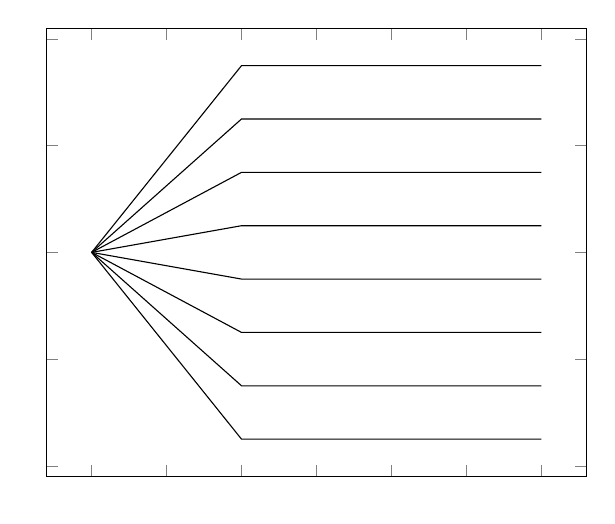
\begin{tikzpicture}
    \begin{axis}[xticklabels={,,},yticklabels={,,}]
      \addplot [color=black] coordinates {
        (1, 0)
        (2, -3.5)
        (3, -3.5)
        (4, -3.5)
      };
      \addplot [color=black] coordinates {
        (1, 0)
        (2, -2.5)
        (3, -2.5)
        (4, -2.5)
      };
      \addplot [color=black] coordinates {
        (1, 0)
        (2, -1.5)
        (3, -1.5)
        (4, -1.5)
      };
      \addplot [color=black] coordinates {
        (1, 0)
        (2, -0.5)
        (3, -0.5)
        (4, -0.5)
      };
      \addplot [color=black] coordinates {
        (1, 0)
        (2, 0.5)
        (3, 0.5)
        (4, 0.5)
      };
      \addplot [color=black] coordinates {
        (1, 0)
        (2, 1.5)
        (3, 1.5)
        (4, 1.5)
      };
      \addplot [color=black] coordinates {
        (1, 0)
        (2, 2.5)
        (3, 2.5)
        (4, 2.5)
      };
      \addplot [color=black] coordinates {
        (1, 0)
        (2, 3.5)
        (3, 3.5)
        (4, 3.5)
      };
    \end{axis}
  \end{tikzpicture}
  % begin of figure 2
  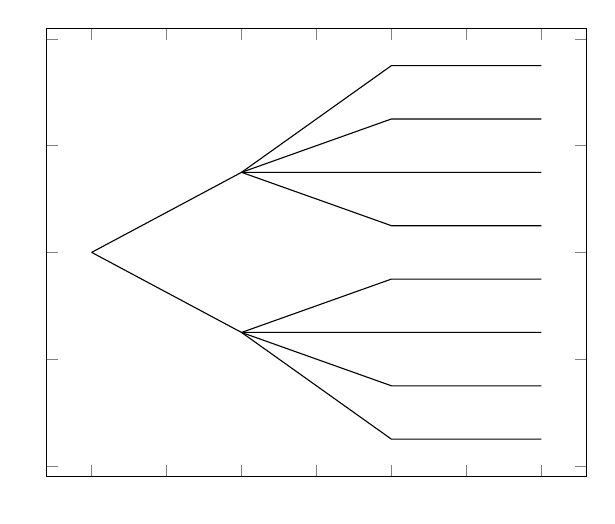
\begin{tikzpicture}
    \begin{axis}[xticklabels={,,},yticklabels={,,}]
      \addplot [color=black] coordinates {
        (2, -1.5)
        (3, -3.5)
        (4, -3.5)
      };
      \addplot [color=black] coordinates {
        (2, -1.5)
        (3, -2.5)
        (4, -2.5)
      };
      \addplot [color=black] coordinates {
        (1, 0)
        (2, -1.5)
        (3, -1.5)
        (4, -1.5)
      };
      \addplot [color=black] coordinates {
        (2, -1.5)
        (3, -0.5)
        (4, -0.5)
      };
      \addplot [color=black] coordinates {
        (2, 1.5)
        (3, 0.5)
        (4, 0.5)
      };
      \addplot [color=black] coordinates {
        (1, 0)
        (2, 1.5)
        (3, 1.5)
        (4, 1.5)
      };
      \addplot [color=black] coordinates {
        (2, 1.5)
        (3, 2.5)
        (4, 2.5)
      };
      \addplot [color=black] coordinates {
        (2, 1.5)
        (3, 3.5)
        (4, 3.5)
      };
    \end{axis}
  \end{tikzpicture}
  % begin of figure 3
  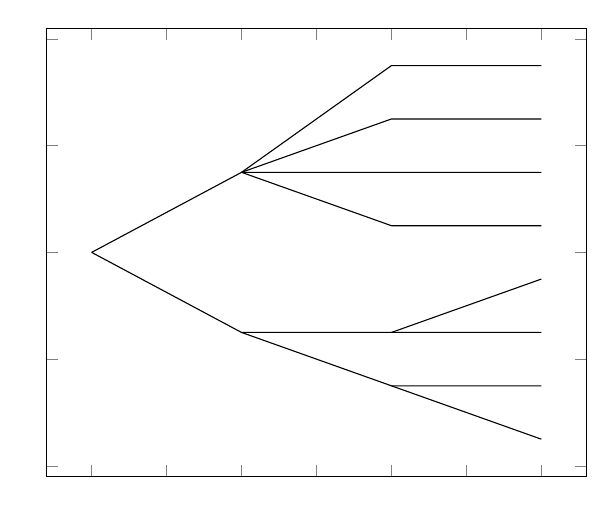
\begin{tikzpicture}
    \begin{axis}[xticklabels={,,},yticklabels={,,}]
      \addplot [color=black] coordinates {
        (3, -2.5)
        (4, -3.5)
      };
      \addplot [color=black] coordinates {
        (2, -1.5)
        (3, -2.5)
        (4, -2.5)
      };
      \addplot [color=black] coordinates {
        (1, 0)
        (2, -1.5)
        (3, -1.5)
        (4, -1.5)
      };
      \addplot [color=black] coordinates {
        (3, -1.5)
        (4, -0.5)
      };
      \addplot [color=black] coordinates {
        (2, 1.5)
        (3, 0.5)
        (4, 0.5)
      };
      \addplot [color=black] coordinates {
        (1, 0)
        (2, 1.5)
        (3, 1.5)
        (4, 1.5)
      };
      \addplot [color=black] coordinates {
        (2, 1.5)
        (3, 2.5)
        (4, 2.5)
      };
      \addplot [color=black] coordinates {
        (2, 1.5)
        (3, 3.5)
        (4, 3.5)
      };
    \end{axis}
  \end{tikzpicture}
  % begin of figure 4
  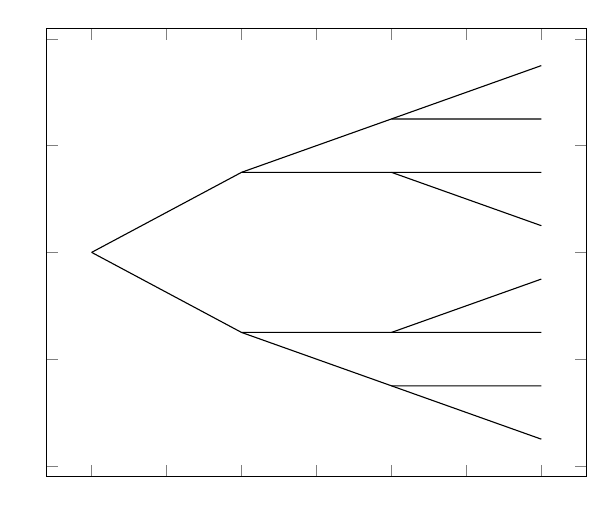
\begin{tikzpicture}
    \begin{axis}[xticklabels={,,},yticklabels={,,}]
      \addplot [color=black] coordinates {
        (3, -2.5)
        (4, -3.5)
      };
      \addplot [color=black] coordinates {
        (2, -1.5)
        (3, -2.5)
        (4, -2.5)
      };
      \addplot [color=black] coordinates {
        (1, 0)
        (2, -1.5)
        (3, -1.5)
        (4, -1.5)
      };
      \addplot [color=black] coordinates {
        (3, -1.5)
        (4, -0.5)
      };
      \addplot [color=black] coordinates {
        (3, 1.5)
        (4, 0.5)
      };
      \addplot [color=black] coordinates {
        (1, 0)
        (2, 1.5)
        (3, 1.5)
        (4, 1.5)
      };
      \addplot [color=black] coordinates {
        (2, 1.5)
        (3, 2.5)
        (4, 2.5)
      };
      \addplot [color=black] coordinates {
        (3, 2.5)
        (4, 3.5)
      };
    \end{axis}
  \end{tikzpicture}
  \caption{Evolution of the stage-wise MILP algorithm for a tree with two branches to each node.
    Top left: The tree is initialized with only the root node.
    Top right: After solving the MILP of the root node.
    Bottom left: After solving the lower of the two second stage nodes.
    Bottom right: The tree, completely solved.
  }
  \label{fig:swmilp-explanation}
\end{figure}
%%% Local Variables:
%%% mode: latex
%%% TeX-master: "da"
%%% End:

\todo[inline]{Describe each step of the algorithm im Freitext}
\todo[inline]{Create mgatex figure that illustrates the meanings of the sets}
\subsubsection{Stochastic Search Solution to Large-Scale MILP}
\todo[inline]{Describe the stochastic search solution}
\todo[inline]{Create an algorithm object for the }
\subsubsection{Results}
In this section, we will evaluate the scenario trees generated with the algorithm of the previous paragraph. As discussed above, the general MILP approach is particularly suitable to problems with a discrete set of outcomes at each stage. Therefore, we will focus on processes with that characteristic feature.

The results in this section were created using an implementation of the above algorithm in C++. The commercial solver Gurobi was employed to solve the MILP subproblems at each stage.  

\paragraph{Coin Toss} Consider the stochastic process created by successive random coin tosses. In order to analyze how well the algorithm does on unknown problems, we will pretend that the only information we have is a black box process that generates one scenario, which is a sequence of 3 successive coin tosses. We, of course, know that the actual probabilities of each state. We will compare the resulting scenario tree with
\paragraph{Log-normal SP}
\begin{itemize}
\item the true solution, to assess the degree of suboptimality
\item with a naive tree generated by random selection of nodes from the set of scenarios. This helps us evaluate whether the extra effort put in to solve the MILP actually improved the prediction of the state.
\end{itemize}
\subsection{NLP Formulation}
In this section, we will present a novel approach to approximating scenario trees. While the previous section was concerned with generating scenario trees for discrete underlying event spaces, continuous event spaces are very common. Obvious examples for stochastic processes with continuos state spaces are prices and demands.

In cases where intermediate values are sensible choices for scenarios, the algorithm described above will sacrifice two possibilities for improvement. First, notice that the general structure of the problem is still given by the same minimum flow problem (\ref{eq:symbolic-optimization-with-minflow2}). The difference to the MILP formulation is the set of feasible trees $\mathcal{T}$. If intermediate values for the states are acceptible, as opposed to only those that were part of the original scenario set, it trivially holds that
\begin{equation}
  \label{eq:T-D-subset-T-C}
  \mathcal{T}_D\subset \mathcal{T}_C,
\end{equation}
where $\mathcal{T}_D$ is the set of feasible trees in the discrete case, and $\mathcal{T}_C$ is the set of feasible trees in the continuous case. It is therefore obvious, that the objective function for the continuous case must be equal to or lower than that of the discrete case. This means, that the continuous formulation allows for a tighter approximation.

The second advantage is the fact, that the continuous problem can be modeled with much fewer variables. This allows us to solve all stages at once, giving us the oportunity to overcome the suboptimality introduced by the stage-wise solution.

Something one does not have to worry about: Given a stochastic distribution that is composed of two hills, some might be worried that the algorithm might create intermediate values. This is, however, not a concern, since an intermediate solution will lead to a higher Kantorovich Distance.

In the following seciton, we will present a derivation of the model used to construct the trees with feasible intermediate values. Along the same lines as the previous section, we will then discuss the computational results. We will discover that the solution of the model with traditional NLP solvers is impossible. The reasons for their failure will be discussed, and a remedy in the form of genetic optimization will be proposed.
\subsubsection{Derivation of the NLP}
We start with the set of original scenarios $I$ with values $\xi_i^t$ and probabilities $p_i$. As before, we assume the structure of the tree to be given. We introduce additional sets $J$ for the scenarios of the trees, $T$ for the set of time steps, and $N$ for the nodes of the tree. The mapping $n:J\times T\rightarrow N$ is defined as the one-to-one mapping from scenarios and time steps to nodes (see figure \ref{fig:abstract-scenario-tree-for-NLP}). In the MILP model, there was no necessity to differentiate between the scenarios and the nodes, because the problem was solved stage by stage, so there was a one-to-one mapping between these two. Here, however, one scenario will always contain multiple nodes, and all nodes except for the leaf nodes will belong to more than one scenario.

The variables in this model are, in general the same as in the abstract model (\ref{eq:symbolic-optimization-with-minflow2}) and the MILP model, but there are some differences due to the structure. The probabilities $q$ of the nodes will not be defined directly over the set of nodes, but the set of scenarios. Given the probabilities of the scenarios, the probability of a node can easily be derived by adding up the probabilities of all scenarios this node belongs to. This definition has the advantage, that the probabilistic relations between nodes are automatically satisfied - for example the condition that the probability of every node has to be equal to the sum of probabilities of its children.  Similarly, the (discretized) measure $\eta_{ij}$ specifies the flow between an original scenario $i \in I$ and a scenario of a tree $j \in J$.

Since the exact values of the tree's nodes are not known beforehand, the distance between the nodes and the original scenarios are not known either. The distance is usually a nonlinear, non-differentiable function. For now, we will replace it with an additional variable $c$, and deal with modelling it farther below. Note that while we think of $c$ as a mapping on $I\times N$, this is - due to the one-to-one mapping induced by $n$ - the same as $I\times J\times T$, which is more convenient.

The objective function is again the Kantorovich functional adopted to the particular tree structure.
\begin{equation}
  \label{eq:NLP-derivation-objective}
  \sum_{i\in I}\sum_{j\in J}\sum_{t\in T} \eta_{ij}\cdot c_{ijt}
\end{equation}
As always, the following properties of the marginal distributions of the measure $\eta$ have to hold:
\begin{eqnarray}
  \label{eq:eta-nlp-marginal-q}
  \sum_{i\in I}\eta_{ij} &=& q_j \;\forall\, j\in J\\
  \label{eq:eta-nlp-marginal-p}
  \sum_{j\in J}\eta_{ij} &=& p_i \;\forall\, i\in I
\end{eqnarray}
As was shown above, these equations already ensure, that the probabilities of the tree's scenarios sum to one. Introducing the bounds
\begin{equation}
  \label{eq:bounds-nlp-q-eta}
  0 \leq \eta,\; 0\leq q
\end{equation}
completes the problem except for the distances $c_{ijt}$.

To model the distances, a metric must be selected. The choice of the best metric depends on the problem belongs to the domain of modeling rather than algorithmic questions that we address here. In the following, we will show how to model the distance $c_{ijt}=c(\xi_i^t,\nu_j^t)$ in the most common norms $\Vert\cdot\Vert_1$, $\Vert\cdot\Vert_2$, and $\Vert\cdot\Vert_\infty$.
%
\paragraph{$\infty$-norm} The one norm is defined as the maximum over the absolute value of all components. 
\begin{equation}
  \label{eq:max-c-definition}
  c_{ijt} = \max\left\{\left|\xi_{id}^t-\nu_{n(j,t)d}\right|,\; d\in D\right\}
\end{equation}
where $D=\left\{1,\, ...,\,n\right\}$ is the set of dimensional indices of the stochastic process. The absolute value can be replaced by the maximum expression
\begin{equation}
  \label{eq:abs-is-a-max}
  \left|\xi_{ik}^t-\nu_{n(j,t)d}\right| = \max\left\{\xi_{ik}^t-\nu_{n(j,t)d},\, \nu_{n(j,t)d}-\xi_{ik}^t\right\}.
\end{equation}
The maximum operator inside the maximum can, of course, be omitted. What is left is the maximum of a finite number of terms. This maximum can be expressed inside the NLP by adding $ |D| \cdot |I|\cdot |J|\cdot |T|$ pairs of inequality constraints of the form
\begin{eqnarray}
  \label{eq:c-as-inftynorm}
  c_{ijt} &\geq& \xi_{id}^t - \nu_{n(j,t)d},\\
  c_{ijt} &\geq& \nu_{n(j,t)d} - \xi_{id}^t.  
\end{eqnarray}
\paragraph{$\mathbf{1}$-norm} Modeling the $1$-norm in the language of inequalities is somewhat more involved, but works basically the same way as the $\infty$-norm. Additional variables $a_{dijt}$ have to be introduced to express the absolute values of the differences in each dimension of each pair, defined by
\begin{eqnarray}
  \label{eq:c-as-1norm-def-a}
  a_{ijtd} &\geq& \left| \xi_{id}^t - \nu_{n(j,t)d}\right| \\
  a_{ijtd} &\geq& \left|  \nu_{n(j,t)d} - \xi_{id}^t\right|
\end{eqnarray}
The distances are then defined by
\begin{equation}
  \label{eq:c-as-1norm}
  c_{ijt} = \sum_{d \in D} a_{ijtd}.
\end{equation}
\paragraph{$\mathbf{2}$-norm} The $2$-norm is much easier to model than the $1$-norm and the $\infty$-norm since the squaring makes the absolute values that give rise to the excessive use of additional inequality constraints. Instead, the distance variables can be defined by the simple equations
\begin{equation}
  \label{eq:c-as-2norm}
  \left(c_{ijt} \right)^2 = \sum_{d \in D}\left( \nu_{n(j,t)d} - \xi_{id}^t \right)^2
\end{equation}
For our purposes, the choice is arbitrary. For the common case of single-valued stochastic processes, the three definitions coincide. In our implementations, we will use the formulation of the $\infty$-norm, since it offers the smallest number of additional variables while at the same time being a linear equation. The $2$-norm has only half the number of equations, but is subject to problems in the scaling and introduces a nonlinearity in the constraints, which seems favourable to avoid.

The discussion closes the derivation of the NLP model for generating scenario trees. The following sections will be dedicated to solving this NLP. In the next esection, experiences with KKT-based solvers is discussed. The solution is found to be problematic, with convergence and local optimality issues. To solve the problem to full optimality, the use of global (heuristic) optimization techniques is explored in the following section.
\subsubsection{Structure of the Optimization Problem}
In this section, the optimization problem derived in the previous section will be restated in its entirety, and its structural properties will be discussed to the degree that it is useful for solving it.
\begin{eqnarray}
  \label{eq:full-nlp-restated-objecive}
  \min_{\eta, q, c}&&  \sum_{i\in I}\sum_{j\in J}\sum_{t\in T} \eta_{ij}\cdot c_{ijt}\\\label{eq:full-nlp-restated-q}
  \mathrm{s.t.}&&\sum_{i\in I}\eta_{ij} = q_j \;\forall\, j\in J\\
  \label{eq:full-nlp-restated-p}
  &&\sum_{j\in J}\eta_{ij} = p_i \;\forall\, i\in I\\
  \label{eq:full-nlp-restated-ineq1}
  &&c_{ijt} \geq \xi_{id}^t - \nu_{n(j,t)d},\\
  \label{eq:full-nlp-restated-ineq2}
  &&c_{ijt} \geq \nu_{n(j,t)d} - \xi_{id}^t\\ 
  &&0 \leq \eta,\; 0\leq q
\end{eqnarray}
The problem is a nonconvex, quadratic optimization problem. For the example of three time steps, the Hessian of the objective function has the structure
\begin{equation}
  \label{eq:structure-of-quadratic-hessian}
  Q = \left[\begin{array}{ccccc}
      0&0&0&I&0\\0&0&0&I&0\\0&0&0&I&0\\I&I&I&0&0\\0&0&0&0&0
    \end{array}\right]
\end{equation}
if the variable ordering is $(c,\eta, q)$. This matrix obviously is not positive definite. In fact, it can be found that the inertia of this matrix, meaning the triple of the numbers positive, negative, and zero variables, is
\begin{equation}
  \label{eq:inertia-of-hessian}
  \left(n, n, T\cdot n\right)
\end{equation}
where $n=|I||J|$, and $T$ is the number of stages (Proof very easy, maybe in appendix?). \cite{Pardalos1991} showed that quadratic optimization problems with at least one negative eigenvalue are $\mathcal{NP}$-hard.
\subsubsection{Solution with local (KKT)-NLP solvers}
In this section, we will discuss the applicability of general purpose KKT solvers to the problem stated above. There are several issues that make this problem particularly hard to solve for KKT based solvers. Among these problems are
\begin{description}
\item[Negative Curvature] KKT solvers use first and second derivatives to generate search directions. Note that KKT points are only stationary points, not guaranteed to be minima of the problem. In the situation of negative curvature, the local maximum is the attractor of Newton's method applied to the KKT-problem. Special care must be taken by the algorithm to reject search directions that lead to a KKT point that is a local maximizer for the objective function
\item[Local Minima] KKT points are an inherently local property of an optimization problem. The only way to find the global optimum is through extensive spatial search. This search can be conducted by applying a deterministic KKT solver to many different, randomly selected starting points.
\item[Large Scale] Due to the complications in modeling the distances $c$, and the fact that using a greater number of original scenarios will always increase the accuracy of the approximation, the solver has to deal with a very large number of variables - typically on the order of one million.
\end{description}
We used the interior point solver IPOPT (\cite{IpoptImplementation2006} as the KKT solver. IPOPT is specifically designed to deal with large-scale non-convex programming problems. It has provisions that ensure global convergence to a KKT point associated with a local minimum under very soft assumptions.

As is to be expected from the theoreticas analysis above, solving the problem from different starting points leads to very different local minima. Figure \ref{fig:different-local-minima-with-ipopt} shows some examples of local minima the algorithm found. In addition to the locality of the solutions, we experienced an unexpectedly slow convergence as the objective value of the iterates approached the optimal solution, with very large primal steps taken by the algorithm. 

The reason for the poor local convergence again lies in the structure of the problem. Consider the conditions derived for locally superlinear convergence of IPOPT given in \cite{Waechter2005}. There, it is stated that, in order to be able to achieve superlinear local convergence, the sufficient second order conditions (SSOC) must hold for the optimal point. 

One condition among these is that at the optimal point $\left(x^*,\lambda^*\right)$ the Hessian of the Lagrangean $\nabla_{xx}^2\mathcal{L}(x^*,\lambda^*)$ is positive definite when projected onto the nullspace of the constraint Jacobian matrix $\nabla c(x^*)^T$. In our specific case of a quadratic objective function with only linear constraints, the Hessian of the Lagrangean is the matrix $Q$ introduced in equation \ref{eq:structure-of-quadratic-hessian}. The constraints are stated in equations \ref{eq:full-nlp-restated-q} through \ref{eq:full-nlp-restated-ineq2}. IPOPT does not deal directly with inequality constraints, so slack variables $s_{1ijt},\,s_{2ijt} \geq 0$ are introduced and equations \ref{eq:full-nlp-restated-ineq1} and \ref{eq:full-nlp-restated-ineq2} restated as
\begin{eqnarray}
  \label{eq:nlp-ineq1-with-slacks}
  c_{ijt} +s_{1ijt}&=& \xi_{id}^t - \nu_{n(j,t)d},\\
  c_{ijt} +s_{2ijt} &=& \nu_{n(j,t)d} - \xi_{id}^t.
\end{eqnarray}
With this reformulation, the SSOC for the problem can be determined by simple algebra: There are $|J|+|I||J|+3*|I||J||T|$ variables in the problem. The number of positive eigenvalues in the Hessian of the Lagrangean is $|I||J|$ (correponds to ``$n$'' in eqn. \ref{eq:inertia-of-hessian}). All remaining $|J|+3*|I||J||T|$ have to be matched by constraints, because each constraint can only eliminate one direction. There are, however, only $2*|I||J||T|+|I|+|J|$ constraints, so that a total of $|I||J||T|-|I|$ variables with eigenvalues of zero remain unmatched. These directions correspond to the distances $c_{ijt}$ which are not acive, e.g. these indices $i,j$ for which $\eta_{ij}=0$. For these distances, the solution is not unique, since any arbitrary feasible value chosen for them will - all else being equal - yield the same value of the objective function. Due to the barrier term that is added to the objective function, those variables $c$ will be driven arbitrarily far away from their bound, which is the behaviour that was observed.
\begin{figure}
  \centering
  \includegraphics[scale=0.6]{sixgraphs}
\caption{Six solutions of the NLP using IPOPT, starting from random starting points. The distribution to be approximated are independent gaussian distributions. The optimal solution would consist of each node placing its child nodes at the }
  \label{fig:different-local-minima-with-ipopt}
\end{figure}

In conclusion it must be stated that this method did not seem sufficient to adress the problem. Due to the abundance of local optima, some kind of global search has to be conducted. However, due to the poor convergence property of the explored algorithm, the local searches are not fast enough to be able to cover the search space in a reasonable time. 

In the next section, global search approaches are discussed, that are able to overcome some of the difficulties we have faced here.
\subsubsection{Escaping local optima: Global Optimization}
\label{sec:nlp-formulation2}
Global optimization approaches can generally be assigned to one of two categories. The first of those two categories is the class of rigorous spatial branch and bound algorithms. These algorithms work on the idea of underestimating the given function on smaller subdomains by convex functions. The problem is solved for the convex underestimator, which yields a lower bound on the objective. This is conducted until the optimality gap is reasonably small. The second approach is to use stochastic optimization algorithms such as genetic optimization and swarm intelligence.

In this section, both of the above approaches will be applied to solve the NLP to full optimality. First, it will be shown that the spatial branch and bound algorithm can for this problem be expressed as an MILP, which makes the solution much more achievable. In the second part, the application of stochastic search routines to the NLP will be discussed.

\paragraph{The global NLP as an MILP} For the current problem, we can actually derive a much smaller search region. From the property proven above (\ref{to-corresponding-proof}), that
\begin{equation}
  \label{eq:restate-eta-either-p-or-0}
  \eta_{ij} = p_i \;\vee \; \eta_{ij}=0,
\end{equation}
we can transform this problem into a selection problem: Find the mapping from $|I|$ to $|J|$ such that the following optimal value of the linear optimization problem
\begin{eqnarray}
  \label{eq:global-NLP-as-MILP-inner-LP}
  &\min\limits_{c,\nu}&\sum_{i\in I}\sum_{j\in J}\eta_{ij}\sum_{t\in T}c_{ijt}\\
  &\mathrm{s.t.}&c_{ijt} \geq \xi_{id}^t - \nu_{n(j,t)d},\\
  &&c_{ijt} \geq \nu_{n(j,t)d} - \xi_{id}^t
\end{eqnarray}
The full problem can be expressed as an MILP using the \textbf{big-M}-formulation. The basic idea is not to use rule \ref{eq:restate-eta-either-p-or-0} directly, but instead set $\eta_{ij}=p_i$ and manipulate $c_{ijt}$ such that it is zero if the selection binary variable $z_{ij}$ is zero. A basic version of this is the model
\begin{eqnarray}
  \label{eq:NLP-as-MILP-full}
  &\min\limits_{z,c,\nu}&\sum_{i\in I}\sum_{j\in J}\sum_{t\in T}p_i\cdot c_{ijt}\\
  &\mathrm{s.t.}&c_{ijt}+ \nu_{n(j,t)d}+M(1-z_{ij} \geq \xi_{id}^t\\
  &&c_{ijt} -\nu_{n(j,t)d} +M(1-z_{ij}\geq - \xi_{id}^t\\
  &&0\leq c_{ijt} \leq M\cdot z_{ij}\\
  \label{eq:NLP-as-MILP-full-bounds}
  &&z_{ij}\in \left\{0,1\right\}
\end{eqnarray}
with a sufficiently large $M$. There are many ways this formulation could be improved. The big-M formulation might be replaced by a convex hull, and symmetry breaking constraints could be introduced, to just name two. However, with several hundred thousand binary variables,  this problem is way out of reach for today's computing technology to solve to full optimality.

Similar to the MILP selection problem in section \ref{sec:MILP-selection-problem}, the problem size can be significantly reduced by decomposing the problem along the time dimension. If only one stage is solved at the same time, the number of binary variables is reduced from $n_I\cdot n_c^{n_s}$ to $n_I\cdot n_c$, where $n_s$ is the number of stages of the problem, $n_c$ is the number of children per node, and $n_I$ is the number of original scenarios, that were selected to belong to the father node. Even though the smaller problem has to be solved much more often ($n_c^{n_s-1}$ times), this approach is at least remotely feasible. The problem to be solved at each stage is exactly the same as the one presented in equations \ref{eq:NLP-as-MILP-full} through \ref{eq:NLP-as-MILP-full-bounds}, with the set $I$ replaced by the subset of the original nodes that the current node's parent node was selected to cover, and the set $J$ encompasses only the nodes of the tree that are children of the current node.

The decomposition of the temporal dimension might, of course, lead to suboptimal solutions. It may well be, that pronounced suboptimalities introduced by this decomposition appear only in pathological examples. Nevertheless, it would be advantageous to have an algorithm, that could solve all stages simultaneosly. In the next section, we will show how stochastic optimization algorithm can achieve this goal.
\paragraph{Stochastic Search Algorithms}
Since the solution of the full scale MILP presented above is not yet a feasible alternative, we will apply a stochastic optimization algorithm to the problem. Stochastic optimization algorithms usually have the following common features;
\begin{itemize}
\item They rely solely on function values.
\item The search path is stochastic
\item They do not attempt to satisfy a descent property
\end{itemize}
As the algorithm only uses function values, and is in general unable to satisfy additional constraints, the search space will be reduced to the set of variables that are in fact free. These variables are the locations $\nu_{jd}^t$ of the tree nodes. The remainig variables that are necessary to evaluate the objective (e.g. the $\eta_{ij}$ will be computed implicitly. This means that the linear programming problem for the Kantorovich Distance has to be solved at each objective function iteration. The objective, as it is posed to the stochastic optimization solver, is
\begin{eqnarray}
  \label{eq:opt-problem-for-stochastic-solver}
  \min_{\nu}&&f(\nu)\\
  \mathrm{with}\; f(\nu)&=\min\limits_\eta &\sum_{i\in I}\sum_{j\in J}\sum_{t\in T}\eta_{ij}c(\nu_j^t,\xi_i^t)\\
  &\mathrm{s.t.}&\sum_{j\in J}\eta_{ij} = p_i\\
  &&0\leq \eta_{ij}
\end{eqnarray}
Note that that the equation
\[
\sum_{i \in I}\eta_{ij} = q_j
\]
is not necessary, since they do not impose any additional restriciton on the choice of $\eta_{ij}$ - they only serve to define the probabilities $q_j$. (The constraint $q_j\geq 0$ can be deduced from $\eta_{ij}\geq 0$.) These probabilities are, however, unnecessary for the evaluation of the objective function. Since $f(\nu)$ will have to be evaluated very often, it is advisable to keep the internal optimization problem as small as possible.

There are several well-studied, stochastic optimization
algorithms available. We chose Particle Swarm Optimization for the
following reasons:
\begin{description}
  \item[swarm] The local optima are located in distinctly different places of the search space. Algorithms that imitate swarm behaviour intuitively act like multiple starting points in this situation
    \item[locality of the search] At every iteration, the inner linear optimization problem must be solved. If the variables $\nu$ are chosen as perturbations of the previous iterate, the solution of the inner LP is likely not to change.
\end{description}

\subsection{Results}
In this section, the results of the different algorithms for tree construction will be compared. To achieve a good basis for comparison, we will first apply all algorithms to the same simple problem to which the optimal solution is known. 
\subsubsection{Results fl}
\subsection{Conclusion}
\section {example problems}
\subsection{pumped hydro}
\subsubsection {Introduction}
The recent developments have shown an emergence of renewable energy sources such as wind and solar. Besides having no carbon emissions, these two forms of power generation share the issue of unpredictable availability. Due to their dependence on the weather, electricity is not necessarily available when needed. The only tool for storing electricity that is currently available are pumped hydro storage plants.

With the liberalization of the electricity markets and the introduction of electricity exchanges (EEX) in Germany and elsewhere, the valuation of power generation assets has been simplified significantly, since all power generating assets (small amounts) can be valued as put options against the electricity spot price.

Because of the stochastic nature of the underlying physics that lead to the formation of the electricity price, 
\subsubsection{Description}
Consider a hydro pumped storage plant. Figure x illustrates the problem the operator has to solve.

The pumped storage hydro power plant is determined by three variables – The flow x that is being pumped into the reservoir, the flow y that is leaving the reservoir, and the reservoir's current level P.  The optimization problem to be solved is the maximization of the expected profit. 
\subsubsection{Mathematical Formulation and analysis}
Given a stochastic process $\xi$, the problem in its complete form is
\begin{equation}
\begin{array}{cc}
\displaystyle \min_{x,y,P} &\displaystyle\int_0^T \int_{\omega \in\Omega}\xi(\omega,t)\left[x(\omega,t)-y(\omega,t)\right]p(\omega,t)d\omega dt\\
s.t.& \displaystyle\frac{\partial P}{\partial t} = \eta x -y\\
&0\leq x \leq x_{\mathrm{max}}\\
&0\leq y \leq y_{\mathrm{max}}\\
&0\leq P \leq P_{\mathrm{max}}\\
&\displaystyle x(\omega, t)\:\mathrm{ is }\:\mathcal{F}_t(\xi)\:\mathrm{ - measurable.}
\end{array}
\end{equation}
The single part of this problem that is causing the most problems is the measurability constraint. 
\newpage
\bibliographystyle{plain}
\bibliography{da}
\end{document}
